


\section{Benchmarks e metodologia de testes}

\subsection{Motivação}

O controlo de redes ao nível do chamado \emph{Control Plane} (protocolos e subsistemas responsáveis
pelo encaminhamento, gestão, optimização das redes) baseia-se, por razões relacionadas
com a necessidade de um elevado desempenho e de simplicidade, em protocolos de coordenação
entre as diferentes componentes de rede (e.g. \emph{switches, routers, controladores \dots}) com
níveis de consistência do tipo ``consistência eventual''. Por essa razão, o estado propagado ou computado
pelas diferentes componentes da rede transita entre estados consistentes,  passando por períodos de
inconsistência mais ou menos prolongados como é comum quando se utilizam protocolos como
OSPF, IS-IS,~\cite{francois2005achieving}, BGP~\cite{bgpConvergence,consensus-bgp},
OpenFlow~\cite{McKeown:2008:OEI:1355734.1355746}.

O trabalho descrito neste documento integra-se num projecto em que se procura substituir esse nível de \emph{consistência eventual}
por protocolos baseados em níveis de consistência com propriedades bem definidas e sem períodos intermédios de
inconsistência, em redes baseadas no paradigma SDN (\emph{Software Defined Networking}). Nomeadamente,
no que diz respeito aos protocolos de troca de estado, eventos e comandos entre componentes. Um dos objectivos do projecto
passa por substituir as funcionalidades em parte desempenhadas pelo protocolo OpenFlow,
por protocolos da mesma natureza que os protocolos usados para replicar estado em sistemas de bases de dados,
numa abordagem como a descrita em~\cite{dbcp}.

Dados os objectivos do projecto, e tendo em consideração que o principal obstáculo a vencer será o de
conseguir responder ao desafio de obter um desempenho adequado, a avaliação realista do desempenho, em redes de média
ou alta complexidade, é de uma grande importância. Para isso serão necessários emuladores de rede recorrendo a
virtualização, dado ser esta a forma mais realista de proceder a essa avaliação.

O sistema a emular deverá ter um elevado número de  \emph{switches, routers,} controladores \dots a
comunicarem intensamente entre si, utilizando protocolos da mesma natureza que os dos sistemas de
bases dados. Para fazer o estudo comparativo da adequação da emulação com base em máquinas
virtuais versus baseadas em {\conts}, revelou-se necessário utilizar um {\bench}
específico, com características bastante diferentes dos em que esses estudos comparativos têm geralmente lugar, \cf Secção~\ref{relacionado}.
Assim, essa aplicação de teste deve ser caracterizada por uma troca intensa de dados entre as diferentes
componentes do sistema, através de protocolos do tipo dos usados em base de dados, e
simultaneamente, executar em cada componente operações também da mesma natureza que as
requeridas pela execução de actualizações de tabelas de bases de dados.

\subsection{Descrição do \textit{benchmark}}

Visando este projecto a comparação das soluções de virtualização de um ambiente distribuído com as características atrás indicadas, foi desenhada de raiz uma aplicação representativa de um sistema dessa natureza. Como indicado na seção \ref{relacionado}, não foi possível utilizar os mesmos {\textit{benchmarks}} que são usados em estudos semelhantes. A aplicação desenvolvida baseia-se num conjunto de nós em que cada nó possui uma base de dados local. Todos os nós têm acesso à base de dados local, como também à base de dados de todos os outros.

Após uma fase de inicialização, cada nó começa a inserir tuplos nas bases de dados de todos os nós, incluindo a sua cópia local. A aplicação termina quando todos os nós tiverem na base de dados local a totalidade dos tuplos inseridos por todos os nós, os quais são necessariamente indênticos.

Ao variar o débito das inserções e o número de nós do sistema distribuído, é possível analisar a capacidade de emulação de uma rede virtual como também observar quais os limites desta.

O servidor onde foram efetuados os \textit{benchmarks} é composto por dois processadores \textit{Intel Xeon E5-2670 v3} a 2.30GHz com 24 núcleos físicos (48 lógicos) cada, 128GB de RAM DDR4 2400MHz. Este executa o {\hiper} VMWare ESXi 6.5.

Para os testes com {\conts}, foi instanciada no mesmo servidor uma VM que permite os testes correrem num ambiente semelhante a um sistema \textit{cloud}, onde os {\conts} executam sobre uma VM instanciada por questões de segurança. As especificações desta VM consistem em 24 \textit{cores} físicos (48 lógicos) e 94GB de RAM. Foi observado que o sistema, durante os testes, não saturava a memória alocada. O sistema de operação da VM onde foram executados os \textit{benchmarks} foi o CentOS 7. Nos {\conts} é usado MySQL 14.14, Python 3.5.3 e como sistema operativo o Debian 9. As versões de MySQL são distintas.

Para os testes de VMs, foram instanciadas tantas VMs quantos os números de nós parametrizados. Cada VM possuía 4 núcleos do CPU e 3 GB RAM. As ferramentas empregues foram: MySQL 15.1, Python 3.4.8 e como sistema de operação CentOS 7.  

Em ambos os ambientes foi implementado um \textit{ramdisk} na diretoria de escrita do MySQL, de forma a eliminar o \textit{overhead} introduzido por leituras e escritas no disco.

\subsection{Funcionamento da aplicação} \label{func}

Os seguintes parâmetros caracterizam uma execução do \bench:

\begin{itemize}
\item Seja $D$ o débito da aplicação, isto é, o número de tuplos gerados por unidade de tempo em cada instância
\item Seja AG o fator de agregação dos tuplos inseridos de uma só vez nas bases de dados remotas
\item Seja $N$ o número de nós que compõe o \textit{benchmark}; a Figura \ref{topologia} ilustra a topologia da rede com $N=6$
\item Seja \textit{master node} o elemento do sistema cujo endereço IP é o menor
\item Seja T um tuplo composto por dois elementos, uma chave aleatória com probabilidade de colisão computacionalmente nula, e um número aleatório de 0 a 100
\end{itemize}

\noindent
A aplicação desenrola-se em 3 fases:

\subsubsection*{Sincronização}
A fase de sincronização possui como objetivo coordenar todas as instân\-cias, visando a entrada sincronizada do sistema no ciclo principal. O processo de sin\-cro\-ni\-za\-ção consiste no estabelecimento de ligações entre os $N$ elementos (formando uma rede em malha). Posteriormente cada nó efetua uma inserção na tabela de coordenação pertencente à base de dados do \textit{master node}.
Em seguida cada nó consulta periodicamente esta tabela. No momento em que o número de entradas for igual ao número de nós, a fase de inicialização termina.

\subsubsection*{Ciclo principal}
O ciclo principal tem como objetivo simular um sistema distribuído que efetua uma grande quantidade de trocas de mensagens continuamente. 
De acordo com o débito $D$, serão gerados tuplos e inseridos na base de dados local. A cada AG inserções locais serão inseridos os mesmos tuplos nas restantes $N - 1$ bases de dados remotas.

\subsubsection*{Finalização}
No final da fase anterior cada nó remove o tuplo inserido durante a fase de sincronização (presente na tabela de coordenação do \textit{master node}). Em seguida irá consultar periodicamente essa tabela até que esta esteja vazia. Atingido este ponto, cada nó termina a sua execução. O benchmark é concluído após todos os nós terminarem.

\begin{figure}[h!]
	\centering
	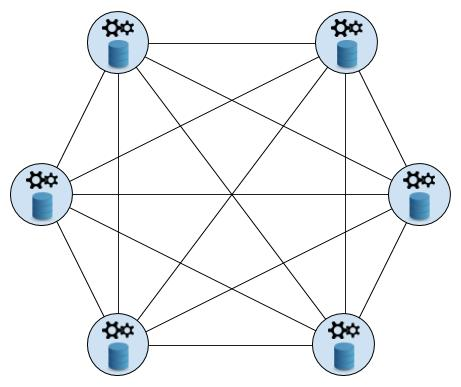
\includegraphics[width=0.6\linewidth]{figures/network_topology.jpg}
	\caption{Topologia da rede do \textit{benchmark} com $N=6$}
	\label{topologia}
\end{figure}


